\chapter{Experimentation}

\textcolor{orange}{we need a paragraph here to briefly explain the experimentation section, what we do here}

\section{ZMQ-based Handover in srsRAN}
\subsection{Objective}
The first phase aims to understand the basics of S1 handover \textcolor{orange}{or we explain what is S1 we assume that it is just handover without the S1} using srsRAN in a controlled simulation. We can use ZMQ and GNU radio to emulate the radio layer. \textcolor{orange}{cite ZMQ and GNU radio? Explain a bit what they are}

\subsection{Approach}

\textcolor{orange}{several bullet points do not have the dot that ends the sentence}

\begin{itemize}
    \item Following \cite{powell_handover_2021}, I started with a pure simulation-based experiment of inducing an S1 handover
    \item This is accomplished by using ZMQ and GNU Radio to simulate the radio layer.
    \item We set up the experiment by running an Open5gs network core, two srsENBs and a srsUE \textcolor{orange}{describe what is srsENB and srsUE}
    \item The eNBs are connected to the network core over the S1AP interface over TCP on my local machine
    \item The eNBs were both connected to the UE using GNU radio and ZMQ, communicating over various TCP ports.
    \item To emulate propagation loss, we add `multiply` blocks on both connections (send and receive) from UE to each eNB, initially setting it to 1 for the eNB we designate as the source cell and 0 for the "target" cell \todo{insert screenshot of GNU flow graph}
    \item On the srsUE process, we collect the measurement logs, fetching the RSRP for both cells
    \item We gradually increase the multiply for the target cell, until the UE is handed over to the target cell
\end{itemize}

\subsection{Results}
\begin{itemize}
    \item Figure \ref{fig:methods:zmq-s1-handover} shows the results of said experiment
    \item As the handover is triggered by default using the A3 Event Trigger, we can see that the A3 offset used in our configuration was 3dBm.
    \item On a static source analysis of the srsRAN code we see the handover occurs when the following condition is met:
$$\text{RSRP}_\text{Target} - \text{RSRP}_\text{Source} > \text{Hysteresis} + \text{A3 Offset} + \text{Of} + \text{Oc}$$
where 
$$\begin{aligned}\text{Of} &= \text{Frequency Offset}_\text{Target} - \text{Frequency Offset}_\text{Source} \\
\text{Oc} &= \text{Cell Offset}_\text{Target} - \text{Cell Offset}_\text{Source}\end{aligned}$$
for the default setup, $\text{Of}=0$ and $\text{Oc}=0$
\item Furthermore, Hysteresis is set to 0, and in our configuration, A3 Offset was set to 3dBm, so we see srsRAN behaving as expected according to the LTE specification.
\end{itemize}
\begin{figure}
    \centering
    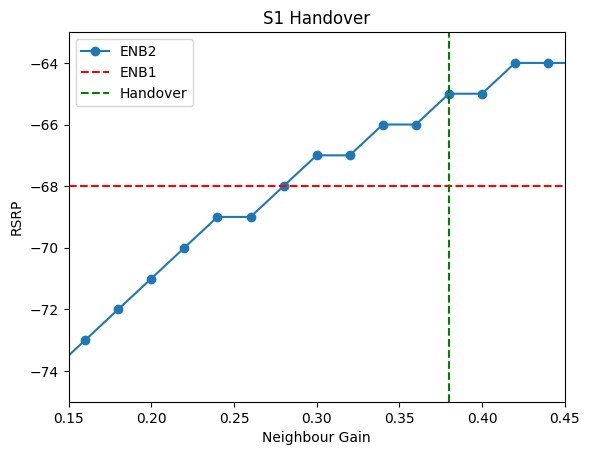
\includegraphics[width=1\linewidth]{src/img/zmq_s1_handover.png}
    \caption{S1 Handover occurring in srsRAN with simulated UE over ZMQ/GNU Radio}
    \label{fig:methods:zmq-s1-handover}
\end{figure}
\subsection{Immediate Discussion}
This phase confirmed srsRAN's adherence to the LTE standard, and a handover was successfully performed in a simulated environment. This phase was limited by the simplistic nature of the simulated radio network, as constants purely dictated network strength. The limited nature of the simulated environment prompted questions about how handovers would occur in more complex environments.

\section{Custom Network Simulator for Large Scale Handovers}
\label{sec:exp:custom}
\subsection{Objective}
Building on the initial findings, this phase was focused on understanding the ping-pong metric and the associated triggers, employing a custom large-scale simulator for analysis.

\subsection{Approach}
Inspired by \citep{hatipoglu_handover-based_2020}, we reconstructed their non-disclosed tool to simulate large-scale handovers.
\begin{itemize}
    \item We look at  to better understand how large-scale handovers are conducted
    \item We replicate their findings to understand what causes ping-pong
    \item Propagation loss was modelled with path shadow loss (insert equations here) \textcolor{orange}{YOU NEED TO DO IT}
    \item UE movement is simulated using a random walk with various speed categories
    \item As the authors did not release the tool they built, we reconstructed the tool, as seen in Figure \ref{fig:methods:grouped-uesim} \textcolor{orange}{explain the figure correctly, what are the axis? What do the colors mean?}
\end{itemize}
\begin{figure}
    \centering
    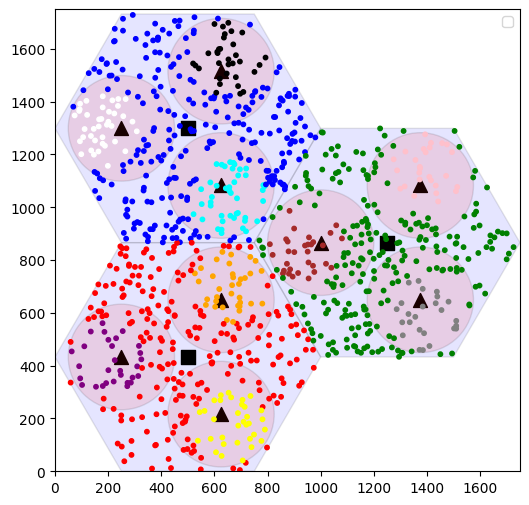
\includegraphics[width=0.75\linewidth]{src//img/grouped_uesim.png}
    \caption{An overview of the 2D simulator}
    \label{fig:methods:grouped-uesim}
\end{figure}
\subsection{Results}
We run the experiment with various handover parameters in Figure \ref{fig:methods:pingpong-uesim}. The impact of the hysteresis value becomes apparent \todo{redo graph showing z-axis} \textcolor{orange}{I miss an explanation of figure 4.3 and the insight of this experiment. Is TTT T(time to trigger) defined somewhere?}
\begin{figure}
    \centering
    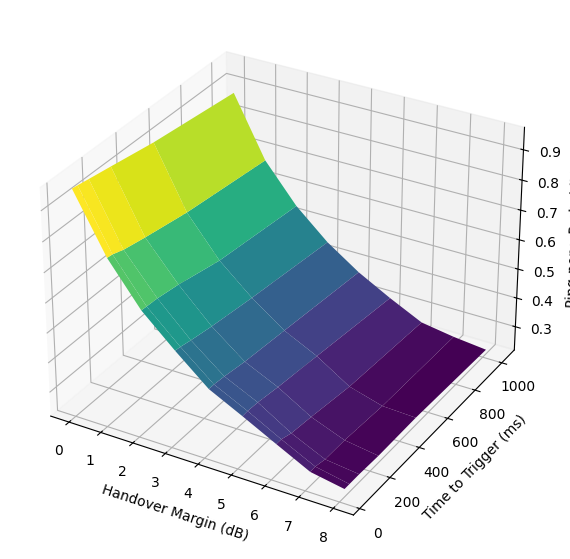
\includegraphics[width=0.5\linewidth]{src//img/pingpong_uesim.png}
    \caption{Ping Pong vs Hysteresis and TTT}
    \label{fig:methods:pingpong-uesim}
\end{figure}
\subsection{Immediate Discussion}
The simulator offered some insights into the conditions that cause ping-pong handovers; however, this was majorly limited by the basic nature of the loss propagation function and highly approximate human movement. This once again reiterates the need for real-world testing to validate these findings \todo{do we validate?}, leading to our next phase of experimentation.


\section{Real-world Network Testbed Implementation}

\subsection{Objective}
After performing the initial experiments in a simulator, we move on to testing in the real world to validate our simulation insights and provide real insight into indoor scenarios. We use a network of radio-enabled srsENBs to examine handover behaviour in a physical environment.

\subsection{Approach}
We plan on performing a range of experiments using the setup described in Sections \ref{sec:research-lab-layout} and \ref{sec:research-software-stack}. These experiments are outlined in the following subsections.

\subsection{Mobility Tests}
\label{sec:exp:real:mobile}
\subsubsection{Objective}
We wish to examine the performance of the indoor handover in various mobility settings.
\subsubsection{Approach}
To reduce confounding variables, we start the network with only two eNBs for this experiment. We examine four different mobility settings:
\begin{itemize}
    \item[\textbf{Stationary}] We set up this experiment by placing the UE machine between the two eNBs and taking care of the environment remaining entirely static; the UE remained stationary, and no persons moved during the experiment. Here, we expect no handover will occur and that the radio signal (as measured by RSRP) will remain constant.
    \item[\textbf{Walking}] We set up this experiment by initially starting the data recording when the UE is near one eNB and then walking towards the other side of the room with the second eNB. Once we reach the eNB, we return to our initial position. To eliminate external factors, no other person was in the lab, and the movement speed was kept roughly constant. We expect the signal strength of the UEs \textcolor{orange}{are we using one UE? Or more?} to vary proportionally to the distance we are from them and expect a handover to occur once we have moved beyond halfway between the UEs. We expect a second handover on the way back.
    \item[\textbf{Rotating}] This experiment was devised to determine the impact of the angle of UE on the corresponding signal strength. We enable two eNBs on the same wall and place the UE halfway between the eNBs in the centre of the room. We slowly rotate the USRP between the two eNBs, back and forth. We expect no significant change in the signal quality, as LOS is not lost, and the distance between the UE and eNBs does not change.
    \item[\textbf{Dynamic Environment}] In this experiment, we aim to test the network's response to a more dynamic environment. The UE is placed in the same position as the \textbf{Rotating} experiment, facing towards the eNBs' midpoint. During the experiment, a person walks in front of the UE and back again, simulating people walking around in a room. We expect some small drop in the signal strength as LOS with the corresponding eNBs is lost, but we believe that signal reflections contribute a sufficient proportion of the signal strength.
\end{itemize}
\subsubsection{Results}
The real-world experiments and the description of the experiment are set out in Figure \ref{fig:methods:real-world-testbed}. \textcolor{orange}{explain further the general idea of the figure. Color represents that the UE is connected to an eNB, if the color changes this means that the UE is associated with another eNBs. Could you also increase the font size of the axis?}
\begin{figure}[p]
    \centering
    \caption{Real-world Network Testbed Implementation: A series of experiments illustrating various aspects of handover behaviour in a real-world setup.}
    \label{fig:methods:real-world-testbed}
    \begin{minipage}{0.45\textwidth}
    \begin{subfigure}{\linewidth}
        \centering
        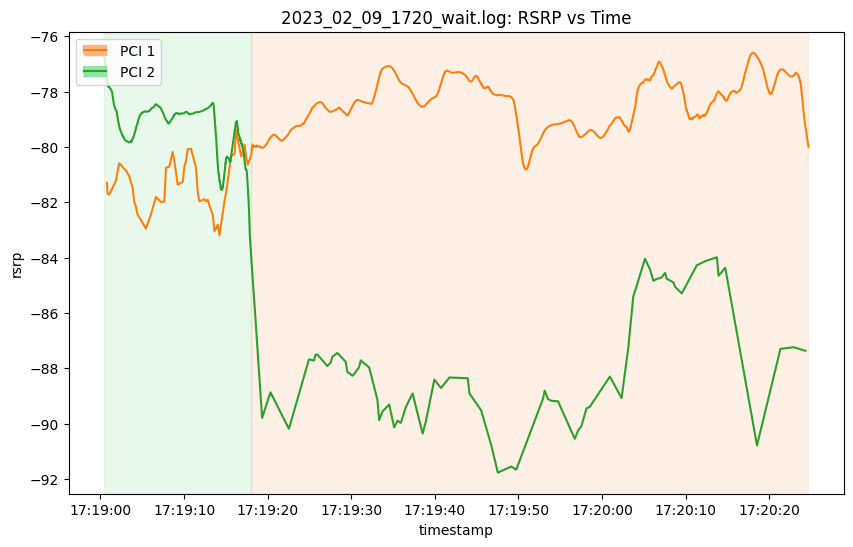
\includegraphics[width=0.9\linewidth]{src//img/2024_02_09_wait.png}
        \caption{Stationary}
        \label{fig:real:mobile:wait}
    \end{subfigure}
    \end{minipage}
    \begin{minipage}{0.45\textwidth}
        \small{Figure \ref{fig:real:mobile:wait}: Shows the effect of no movement on RSRP measurements, indicating the presence of environmental noise and its potential impact on handover decisions.}
    \end{minipage}
    
    \vspace{1cm}
    \begin{minipage}{0.45\textwidth}
    \begin{subfigure}{.9\linewidth}
        \centering
        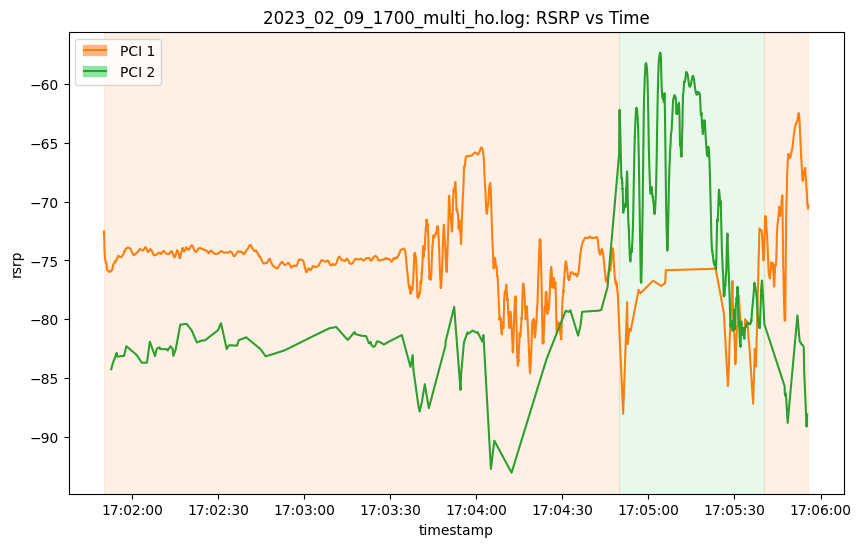
\includegraphics[width=0.9\linewidth]{src//img/2024_02_09_multiho.png}
        \caption{Walking back and forth}
        \label{fig:real:mobile:walk}
    \end{subfigure}
    \end{minipage}%
    \begin{minipage}{0.45\textwidth}
        \small{Figure \ref{fig:real:mobile:walk}: Demonstrates the RSRP and connected cell for a walking back and forth episode. This experiment showcases the dynamic RSRP changes as the UE moves closer or further from each eNB.}
    \end{minipage}
    
    \vspace{1cm}
    \begin{minipage}{0.45\textwidth}
    \begin{subfigure}{\linewidth}
        \centering
        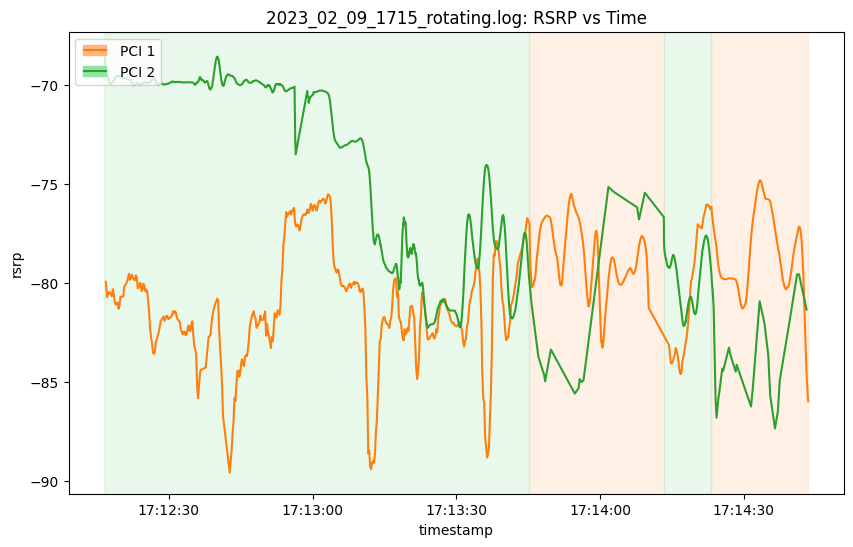
\includegraphics[width=0.9\linewidth]{src//img/2024_02_09_rotating.png}
        \caption{Rotating UE}
        \label{fig:real:mobile:rotate}
    \end{subfigure}
    \end{minipage}
    \begin{minipage}{0.45\textwidth}
        \small{Figure \ref{fig:real:mobile:rotate}: Illustrates the impact of rotating the UE on RSRP fluctuations and handover events, highlighting the sensitivity of handover mechanisms to device orientation.}
    \end{minipage}
    
    \vspace{1cm}
    \begin{minipage}{0.45\textwidth}
    \begin{subfigure}{\linewidth}
        \centering
        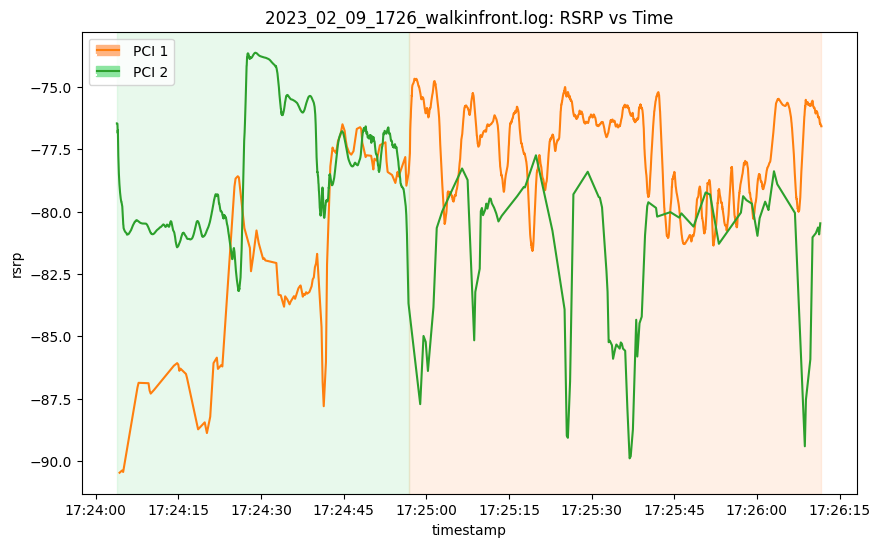
\includegraphics[width=0.9\linewidth]{src//img/2024_02_09_los_block.png}
        \caption{LOS Blockage by walking around}
        \label{fig:real:mobile:block}
    \end{subfigure}
    \end{minipage}
    \begin{minipage}{0.45\textwidth}
        \small{Figure \ref{fig:real:mobile:block}: Examines the effects of line-of-sight (LOS) blockage by simulating movement around the UE. This scenario reflects real-world dynamics where human movement can influence signal quality and handover behaviour.}
    \end{minipage}
\end{figure}
\subsubsection{Immediate Discussion}
These findings underscored the complexity of indoor scenarios.

Figure \ref{fig:real:mobile:wait} shows the high impact of environmental noise even in stationary situations \textcolor{orange}{explain it more we expected no change on the RSRP but is not the case. We observe that even in stationary environments, there is a big change in the RSRP, and this triggers handover. Explain why this is happening, any interesting finding is appreciated, we need to show the reader anything relevant}. Figure \ref{fig:real:mobile:walk} performs handovers as a UE moves closer and further from a target cell as expected \textcolor{orange}{Explain it further, the UE moves linearly between the eNBs, we expect the RSRP to behave in this way (the RSRP does it? It seems that RSRP does not change smoothly). There is a handover once the UE approaches the second eNBs and another once it gets further. }. However, the large noise spikes were not accounted for in the expectations of the experiment. The following experiment in Figure \ref{fig:real:mobile:rotate} seeks to highlight this possible disparity by rotating the UE back and forth, causing significant disturbances to RSRP \textcolor{orange}{explain it further, why do we have 3 handovers? Does this make sense? Please talk about the figure and provide some insight if possible}. Finally, Figure \ref{fig:real:mobile:block} highlights further issues caused by the dynamic environment \textcolor{orange}{the same with this figure}.

The four experiments together highlight the high difficulty of indoor handover. \textcolor{orange}{Talk more of the general idea, the RSRP changes quickly and it does not behave as expected. This challenges indoor handover. You need to provide more details}

\subsection{Handover Impact on Latency}
\label{sec:handover-impact}
\subsubsection{Objective}
To understand the level of the issues found in the previous experiment must be mitigated, through which unnecessary handovers are reduced, we must understand the impact on metrics such as throughput and latency of the connection. This experiment focuses on the latency introduced by an individual handover.

\subsubsection{Approach}
To determine the latency impact of a handover event, we utilise ICMP \texttt{ping} messages. We setup the UE to have ping messages sent to the EPC every 10ms. We simultaneously use \texttt{tcpdump}\insertref to capture all incoming and outgoing packets. We then can use Wireshark\insertref to analyse the return trip time (RTT). We use Wireshark's inbuild graphing tool to produce a time series of the maximum RTT.

% \begin{itemize}
%     \item To determine the actual impact of a handover, we must measure it quantitatively
%     \item We run a ping flood from the UE to the EPC and capture the packets using `tcpdump`
%     \item Similarly to the previous experiment, we walk from one eNB to another to induce handover
%     \item The packet traces are then analysed with Wireshark to see the latency of each packet. We perform a rolling max smoothing with a window size of 2ms.
%     \end{itemize}

To capture a handover event, we set up the experiment similarly to Section \ref{sec:exp:real:mobile}'s walking experiment, walking from one eNB to the other.
\subsubsection{Results}
The results are shown in Figure \ref{fig:methods:ping-handover}
\begin{figure}
    \centering
    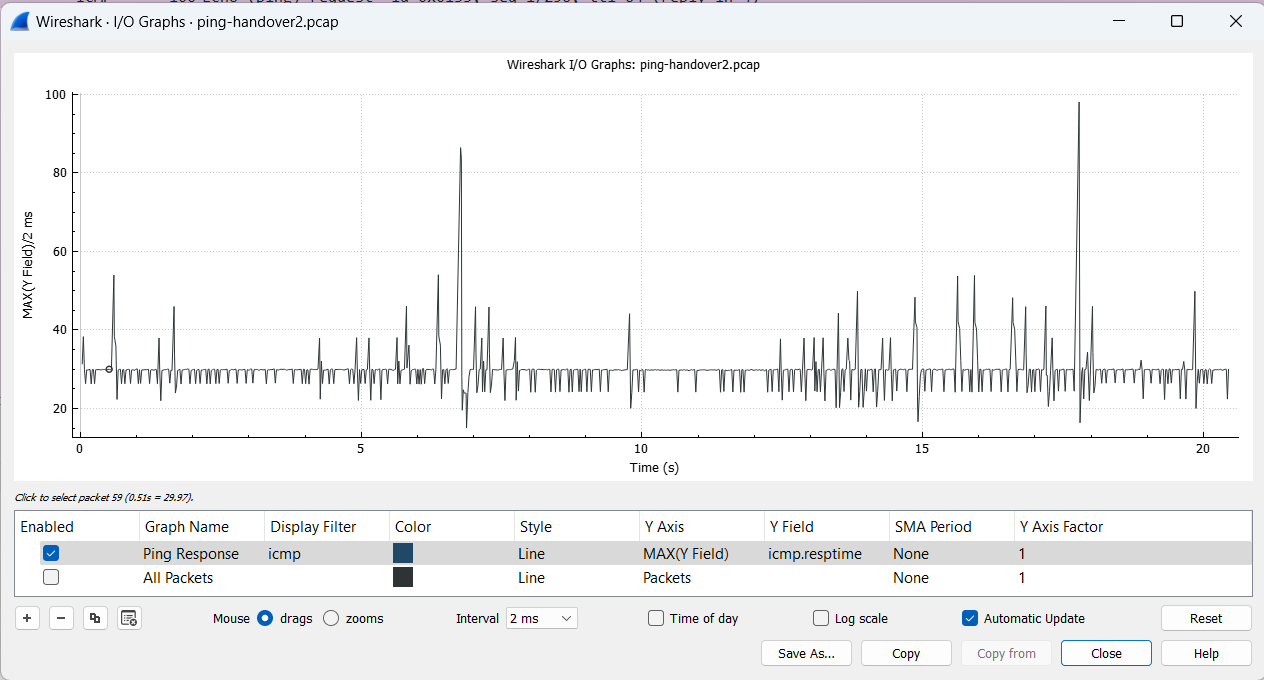
\includegraphics[width=0.75\linewidth]{src//img/ping-handover.png}
    \caption{Wireshark view of Ping during a handover event \textcolor{orange}{we need to make this figure bigger, y-axis is not well recognized}}
    \label{fig:methods:ping-handover}
\end{figure}
\subsubsection{Immediate Discussion}
We see a large latency spike during the handover event, however no packets are dropped due to the EPC/eNB buffering any packets received during HO. We can see that the latency maxes out at 96ms. This result is consistent with \citet{zhang_performance_2012}.

\subsection{Handover Impact on Throughput}

\textcolor{orange}{this subsection does not evaluate datarate for handover since the handover is not triggered in any of the two figures, 4.6 and 4.7. Raname by Throughput analysis in indoor environments?}

\subsubsection{Objective}
To further understand the impact of handover in indoor environments, we must also examine the throughput drop due to handover. This section focuses on repeating the mobility tests in Section \ref{sec:exp:real:mobile} while measuring throughput.

\subsubsection{Approach}
To measure the impact on throughput during a handover event, we must first determine an approach. We have two options in communication protocol: UDP and TCP. UDP, a best-effort protocol, contains no rate limiting or reliable message delivery; however, it can deliver the highest throughput. Conversely, TCP ensures reliable message delivery and varies the transmission bandwidth depending on packet loss. It also accounts for the majority of internet traffic. 

We can use the \texttt{iperf3} tool, a network performance tester, as it is the most popular software. It also allows both UDP and TCP testing.

\begin{itemize}
    \item We can set up the experiment by enabling all our eNBs and using our lab machine as a UE. We keep the environment and UE static during the experiment.
    \item We start an \texttt{iperf3} server on the EPC. Simultaneously, we begin a \texttt{tcpdump} process to capture all incoming packets
    \item For testing UDP throughput, we start a client on the UE in UDP mode. We set the bandwidth to 100Mbits/s to saturate the uplink.
    \item For TCP testing, we start the client in TCP mode. The bandwidth is automatically determined by the TCP protocol.
    \item We can then measure the throughput by examining the lengths of the incoming packets.
\end{itemize}
\subsubsection{Results}
Figure \ref{fig:4udp} shows a 30-second capture of UDP throughput. The RSRP values remain very constant however the throughput is very erratic. \textcolor{orange}{make figure bigger}

Figure \ref{fig:4tcp} shows 30 seconds of TCP throughput capture. The RSRP values are slightly different. However, the connected eNB has a higher signal strength than the UDP. The throughput is much more constant - due to the TCP rate limiting the connection. However, it transmits at a much lower rate than the UDP connection. Furthermore, there are connection failures lasting more than 2.5 seconds. \textcolor{orange}{any guess why this happens?}
\begin{figure}
    \centering
    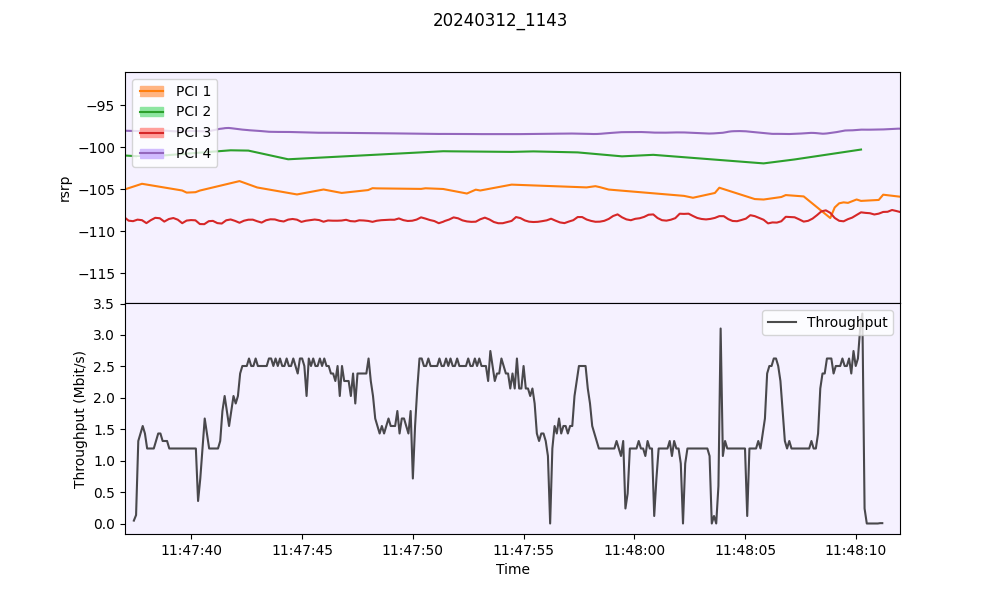
\includegraphics[width=0.5\linewidth]{src//img/4stationary_udp.png}
    \caption{Enter Caption}
    \label{fig:4udp}
\end{figure}
\begin{figure}
    \centering
    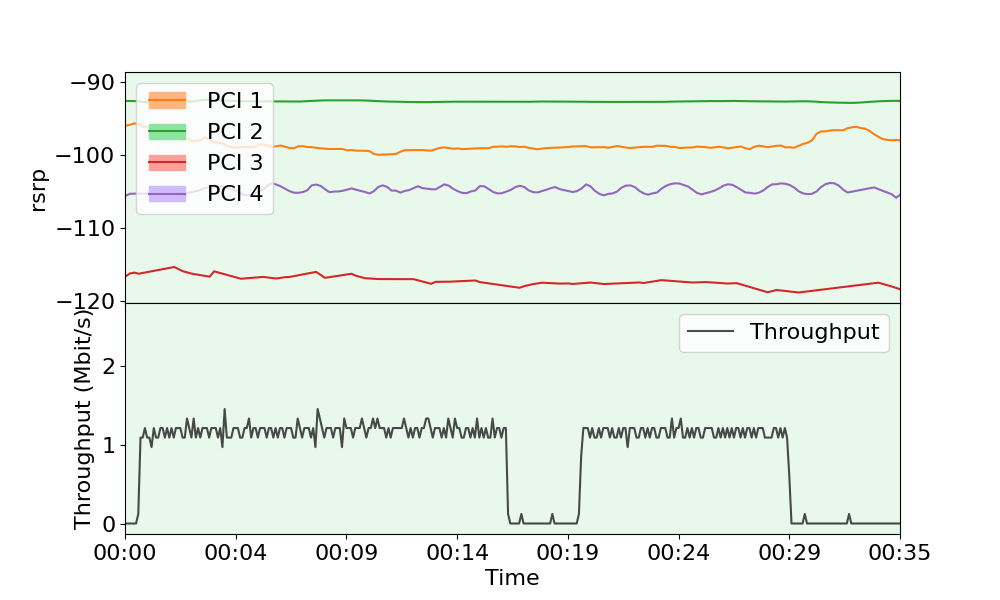
\includegraphics[width=0.5\linewidth]{src//img/4stationary_tcp.png}
    \caption{Enter Caption}
    \label{fig:4tcp}
\end{figure}

\subsubsection{Immediate Discussion}
Determining the best protocol to use for testing the network proves difficult. UDP provides a better understanding of the maximum throughput the connection can allow. However, TCP better emulates how regular communication affects the network.
Due to the network's inherent instability, TCP becomes a nonviable means of testing our network. As packet loss impacts TCP's communication ability, large gaps appear during our throughput measurements. This would limit our understanding of the effect of HO on throughput. Furthermore, we wish to test the network's maximum capacity, and so UDP provides a more granular view.

We, therefore, use UDP in our following experiments.

\subsection{Increasing cell density}
\tocomplete{}

\subsubsection{Objective}
The previous mobility tests were run with only two eNBs enabled. This is not representative of planned indoor deployments; instead, much higher cell density is expected \insertref \textcolor{orange}{that might be partially true, it will depend on the requirements}. This experiment focuses on the performance of the network with a higher number of active cells. We can hypothesise that with increasing cell density (more eNBs enabled) the rate of handover will be much higher.
\subsubsection{Approach}
We perform two sets of experiments, walking and stationary.
\begin{itemize}
    \item We start the experiment in the same way as the last. However, we enable all four eNBs.
    % \item We start a UDP iPerf3 server on the network core, and a client sending 100Mbits/s on the UE, to saturate the throughput
    % \item We capture incoming packets on the network core and use the volume of packets to measure throughput
    % \item We perform three experiments, a stationary one and two random walks through the lab.
    \item We smooth out the RSRP values with a moving average window of 1000ms% and the throughput values over 100ms.
\end{itemize}
\subsubsection{Results}
Results of the experiment are shown in Figures \ref{fig:real:4enb:stationary} and \ref{fig:real:4enb:walk}. \textcolor{orange}{I would not include Figure 4.8 since it is static and we do not have any handover while before we observed handover in static settings, so I would not include it. Please, explain Figure 4.9. The second subfigure seems to be longer and explains it. Explain the small handover, the handovers that last a few milliseconds.}

\begin{figure}
    \centering
    \includegraphics[width=0.75\linewidth]{src//img/4enbEx1Stationary.png}
    \caption{Stationary Capture of Thoughput}
    \label{fig:real:4enb:stationary}
\end{figure}
\begin{figure}
    \centering
    \caption{Moving Capture of Thoughput}
    \label{fig:real:4enb:walk}
    \begin{subfigure}{\linewidth}
        \centering
        \includegraphics[width=0.75\linewidth]{src//img/4enbEx2RandomWalk.png}
        \caption{Capture 1}
        \label{fig:real:4enb:walk1}
    \end{subfigure}
    \begin{subfigure}{\linewidth}
        \centering
        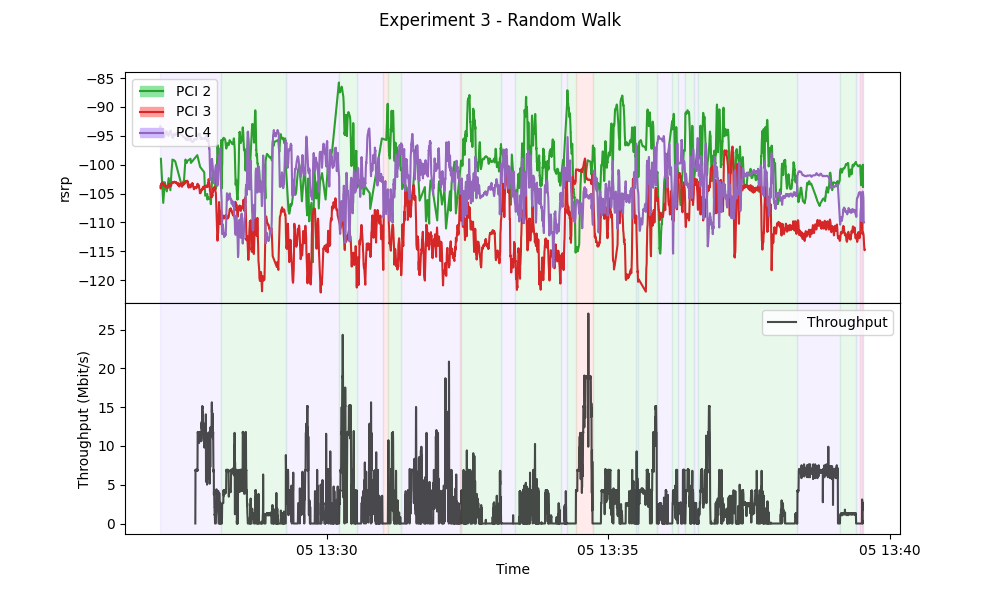
\includegraphics[width=0.75\linewidth]{src//img/4enbEx3RandomWalk.png}
        \caption{Capture 2}
        \label{fig:real:4enb:walk2}
    \end{subfigure}
    \begin{subfigure}{\linewidth}
        \centering
        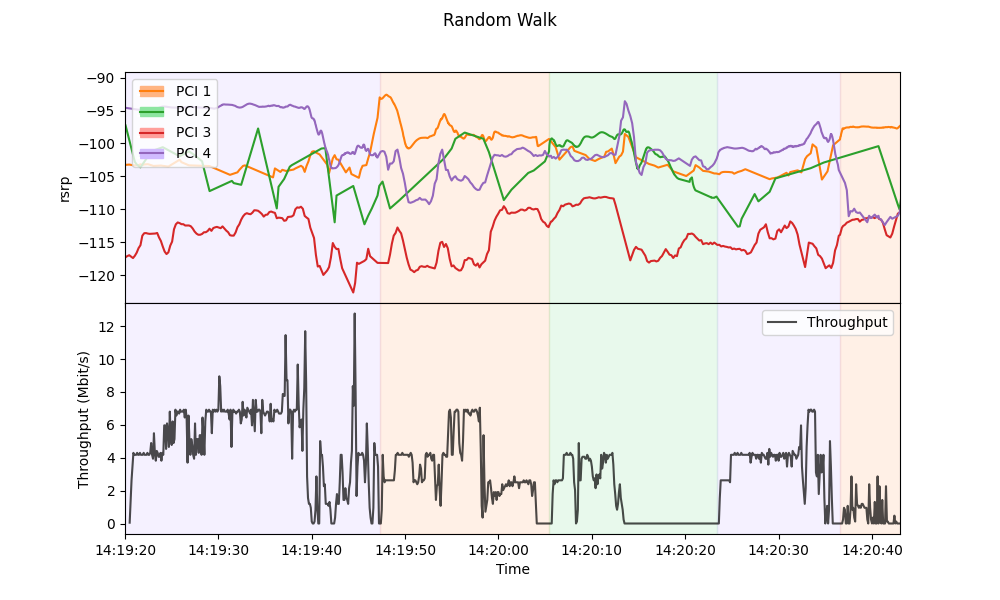
\includegraphics[width=0.75\linewidth]{src//img/4enbEx4RandomWalk.png}
        \caption{Capture 3}
        \label{fig:real:4enb:walk3}
    \end{subfigure}
\end{figure}

% \begin{figure}[p]
%     \centering
%     \caption{High Cell Density experiments: A series of experiments highlighting the increase HO-rate with more cells deployed}
%     \label{fig:real:4enb}
%     \begin{minipage}{0.45\textwidth}
%     \begin{subfigure}{\linewidth}
%         \centering
%         \includegraphics[width=0.9\linewidth]{src/img/4enbEx1Stationary.png}
%         \caption{Stationary}
%         \label{fig:real:4enb:stationary}
%     \end{subfigure}
%     \end{minipage}
%     \begin{minipage}{0.45\textwidth}
%         \small{Figure \ref{fig:real:4enb:wait}: Shows the effect of no movement on RSRP measurements. Against expectations, the signal remains fairly constant}
%     \end{minipage}
    
%     \vspace{1cm}
%     \begin{minipage}{0.45\textwidth}
%     \begin{subfigure}{.9\linewidth}
%         \centering
%         \includegraphics[width=0.9\linewidth]{src/img/4enbEx2RandomWalk.png}
%         \caption{Walking capture}
%         \label{fig:real:4enb:walk1}
%     \end{subfigure}
%     \end{minipage}%
%     \begin{minipage}{0.45\textwidth}
%         \small{Figure \ref{fig:real:4enb:walk1}: Of note, at 13:07:57, we see a ping pong handover that lasts only 57ms. Handover rate is 2.29 handovers/minute}
%     \end{minipage}
    
%     \vspace{1cm}
%     \begin{minipage}{0.45\textwidth}
%     \begin{subfigure}{\linewidth}
%         \centering
%         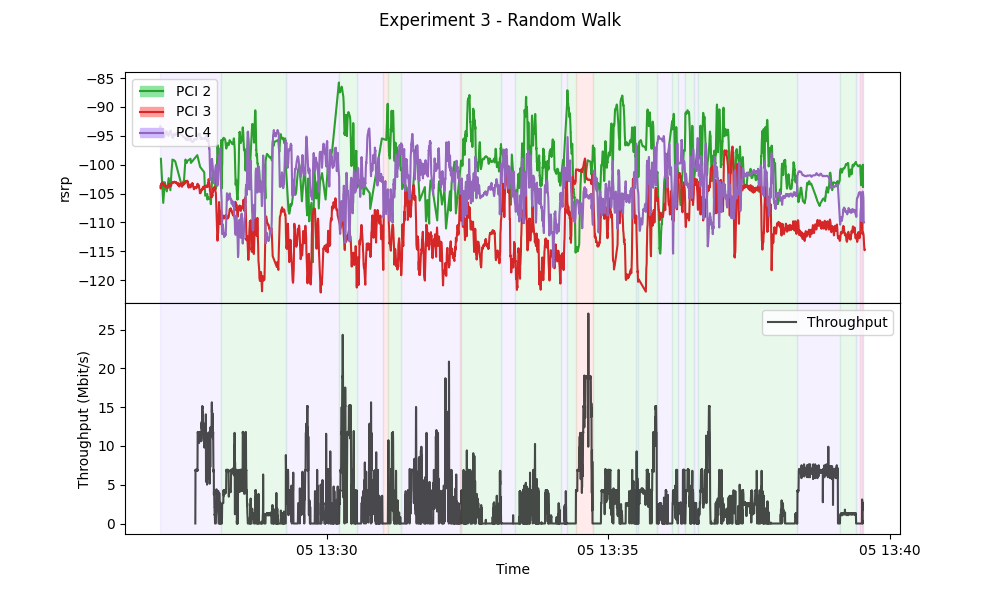
\includegraphics[width=0.9\linewidth]{src//img/4enbEx3RandomWalk.png}
%         \caption{Walking capture}
%         \label{fig:real:4enb:walk2}
%     \end{subfigure}
%     \end{minipage}
%     \begin{minipage}{0.45\textwidth}
%         \small{Figure \ref{fig:real:4enb:walk2}: Handover rate is 2.29 handovers/minute}
%     \end{minipage}
    
%     \vspace{1cm}
%     \begin{minipage}{0.45\textwidth}
%     \begin{subfigure}{\linewidth}
%         \centering
%         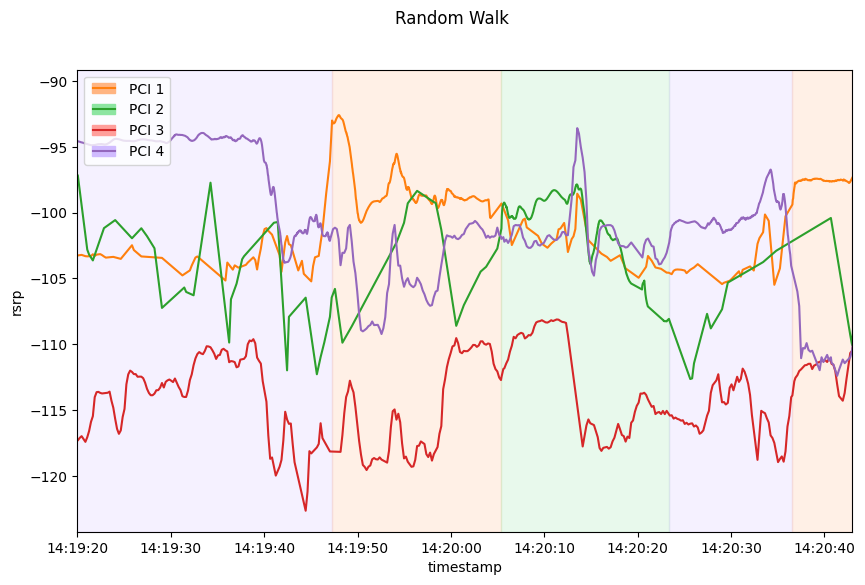
\includegraphics[width=0.9\linewidth]{src//img/real_4enb_walk3.png}
%         \caption{Walking capture}
%         \label{fig:real:4enb:walk3}
%     \end{subfigure}
%     \end{minipage}
%     \begin{minipage}{0.45\textwidth}
%         \small{Figure \ref{fig:real:4enb:walk3}: Handover rate is 2.89 handovers/minute}
%     \end{minipage}
% \end{figure}


\subsubsection{Immediate Discussion}
\begin{itemize}
    \item We see a high rate of handover, even when signal quality has not significantly fallen
    \item To properly understand, we must capture the throughput to see the impact of handovers.
    % \item For better analysis, we instead will attempt to use a TCP iperf3 server to utilise the more reliable protocol to control data flow.
    % \item Handovers occur fairly often, though, but none are under the 1-second threshold for ping pong handover.
    \item For the second walk, eNB with the PCI of 1, dropped off, a very common occurrence in the testing of the network - highlighting the difficulties of maintaining a network
\end{itemize}


% ===========================End Varying Cell Density================================ %



\subsection{Hysteresis Impact}
\tocomplete{}
\subsubsection{Objective}
During the previous experiments, we saw a very high rate of handovers, even when throughput was not improved. We turn to our tuneable parameters of handover, TTT and hysteresis. Considering our results in Experiment \label{sec:exp:custom}, we can hypothesise that \textit{Hysteresis} will most impact our ping-pong and handover rate.

\subsubsection{Approach}
To determine the effect of hysteresis on handover, we run a series of experiments adjusting the hysteresis value. We can set up the experiment with 4 eNBs enabled and the UE stationary, positioned so that the RSRP values of the eNBs are similar, where the chance of a ping-pong handover is high. We run the experiment with hysteresis values of 0, 3dBm, 6dBm and 9dBm.

\subsubsection{Results}
The experiment results are plotted in Figure \ref{fig:methods:hysteresis}. We see the rate of handover decrease for each increase in the threshold. \textcolor{orange}{explain why this happens, hysteresis is designed to avoid ping pong, so if hysteresis is higher we have less handover. But what are the drawbacks of higher hysteresis values? Maybe we push the handover to be triggered too late. Please, talk about it and provide some insight. Maybe refer to the equation where the hysteresis is explained? Or include the equation here for the shake of understanding}

\begin{figure}[p]
    \centering
    \caption{Hysteresis values effects on HO rate}
    \label{fig:methods:hysteresis}
    \begin{subfigure}{\linewidth}
        \centering
        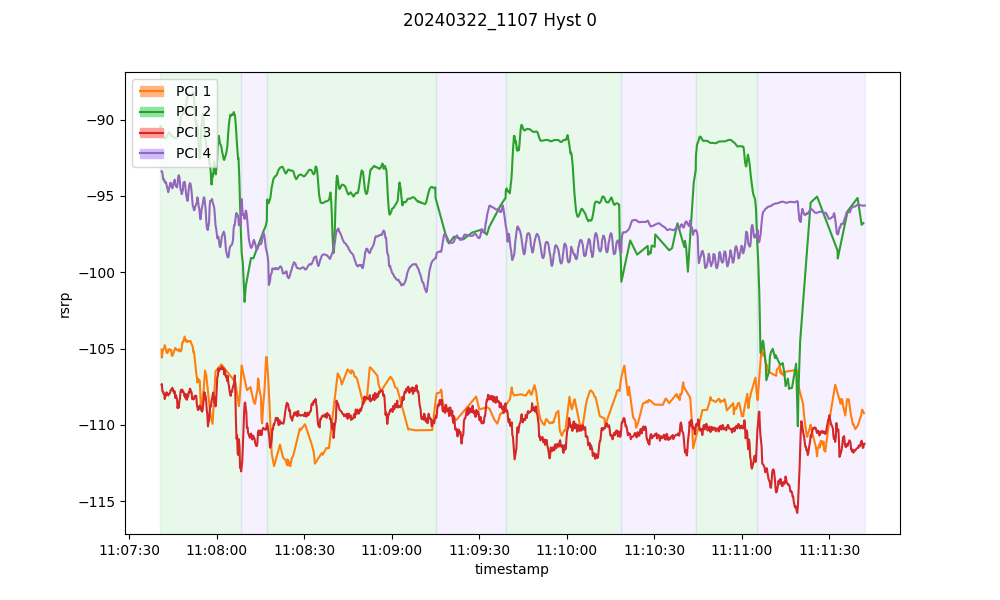
\includegraphics[width=0.6\linewidth]{src//img/5hyst0.png}
        \caption{Hysteresis Threshold: 0dBm}
        \label{fig:methods:hyst0}
    \end{subfigure}
    
    \begin{subfigure}{.9\linewidth}
        \centering
        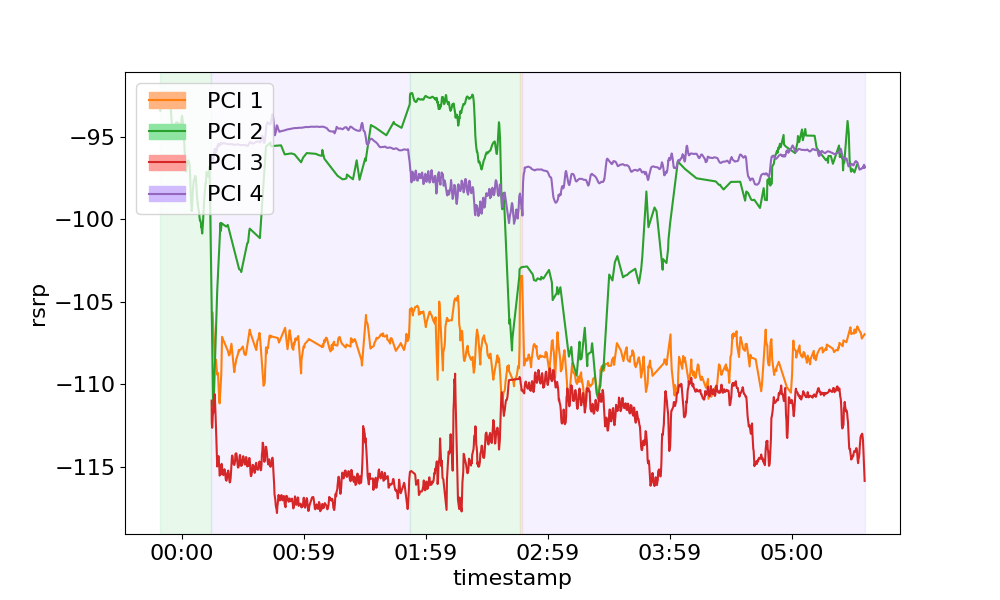
\includegraphics[width=0.6\linewidth]{src//img/5hyst3.png}
        \caption{Hysteresis Threshold: +3dBm}
        \label{fig:methods:hyst3}
    \end{subfigure}
    
    \begin{subfigure}{\linewidth}
        \centering
        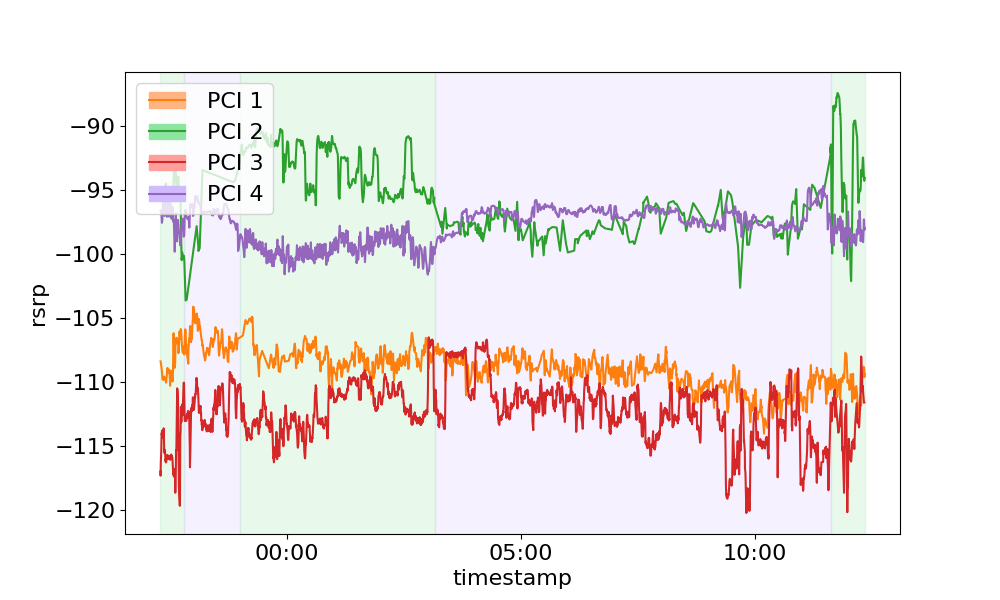
\includegraphics[width=0.6\linewidth]{src//img/5hyst6.png}
        \caption{Hysteresis Threshold: +6dBm}
        \label{fig:methods:hyst6}
    \end{subfigure}
    
    \begin{subfigure}{\linewidth}
        \centering
        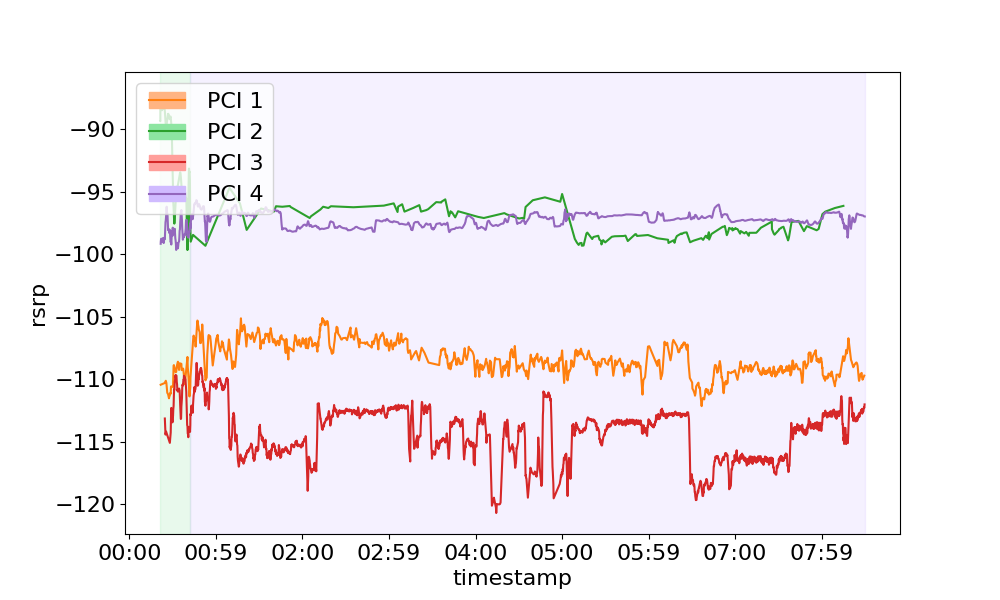
\includegraphics[width=0.6\linewidth]{src//img/5hyst9.png}
        \caption{Hysteresis Threshold: +9dBm}
        \label{fig:methods:hyst9}
    \end{subfigure}
\end{figure}

\subsubsection{Immediate Discussion}
We can conclude that choosing a higher hysteresis value greatly reduces the handover rate.